\documentclass[border=2mm]{standalone}
\usepackage{physics}
\usepackage{tikz}
\usepackage{pgfplots}
\begin{document}
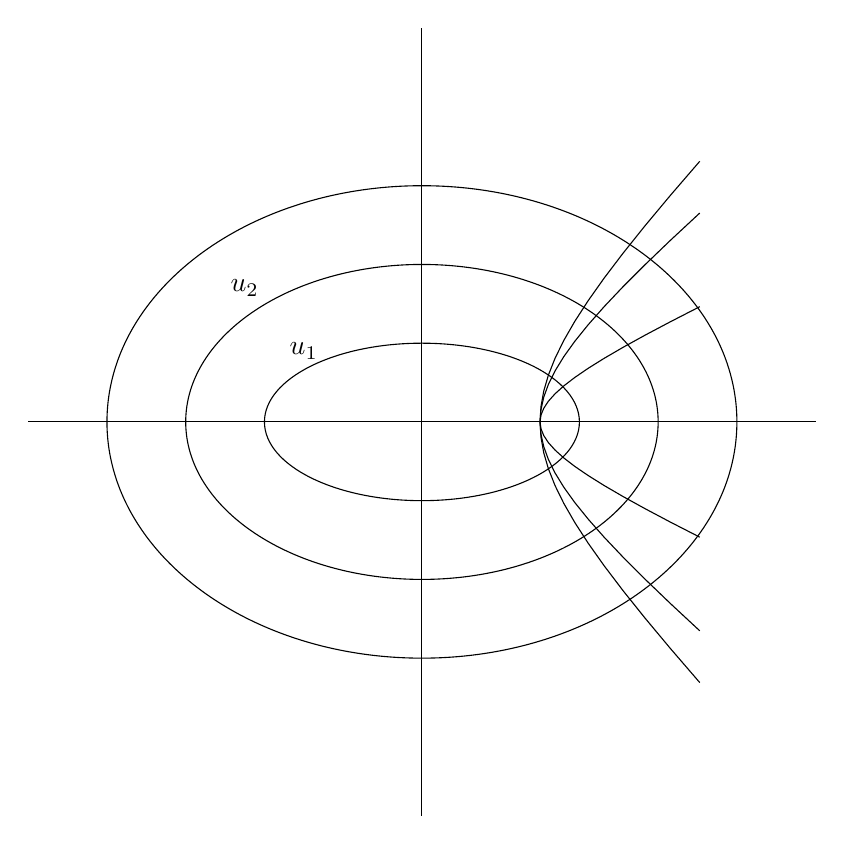
\begin{tikzpicture}
    \draw (-5, 0) -- (5, 0);
    \draw (0, 5) -- (0, -5);
    \draw (0, 0) ellipse (2cm and 1 cm);
    \draw (0, 0) ellipse (3cm and 2 cm);
    \draw (0, 0) ellipse (4cm and 3 cm);
    \node at (-1.5, 0.9) {$u_{1}$};
    \node at (-2.25, 1.7) {$u_{2}$};

    %\pgfmathsetmacro{\e}{1.44022}   % eccentricity
    \foreach \e in {1.44022, 1.3, 1.1}
        {
        \pgfmathsetmacro{\a}{1.5}
        \pgfmathsetmacro{\b}{(\a*sqrt((\e)^2-1)} 
        \draw plot[domain=-1.5:1.5] ({\a*cosh(\x)},{\b*sinh(\x)});
        }
\end{tikzpicture}
\end{document}